\chapter{Single Epidemic Fitting}
\label{ch:single}

In this section we explore the theory and implementation behind a
model fitting framework for single SIR models with unknown
parameters. To provide a simulation of real time model fitting, we
iteratively fit a new, independently optimised model at each data point. Firstly, a
least-squares fitting procedure is implemented in R for a single SIR
epidemic where beta and gamma are assumed to be entirely
unknown. We then extend the implementation to include the number of
initial susceptible individuals, S0; the start time
of the epidemic, t0; and the initial number of infected individuals, I0. This also raises
the issue of epidemic outbreak detection and candidate model selection, which we
will revisit in section SECTIONNNN!. We go on to use a maximum
likelihood based approach which allows for the generation of
confidence intervals. Finally, we reimplement the above approaches in
C++ to provide a much faster fitting framework.

\section{Epidemic Data}
The data that we wish to characterise is the change in number of
infected individuals over time. In this context, the term `infected individuals' may be
defined as individuals infected with a disease, or individuals that
have viewed a particular \emph{YouTube} video or `liked' a particular
\emph{Facebook} post. Examples of this type of data are shown in
Figure~\ref{figure:examples}. \emph{R} is ideally suited for the easy management and
manipulation of data through the use of the `data frame' type. In C++,
we import data as .csv files and carry out all manipulation and use
using vectors.


\begin{center}
\begin{figure}[ht!]

\includegraphics[width=15cm]{simplesir.png}
\caption{Example synthetic epidemic data generated using the
  \emph{GillespieSSA} algorithm in \emph{R}. In this model: $beta =
  0.0015, gamma = 0.1, S0 = 800, I0 = 1$.}
\label{figure:examples}
\end{figure}  
\end{center}

We use the results of solving ODEs with known parameters and
independent runs of the \emph{GillespieSSA} algorithm to test the
framework's ability to find the true model
parameters. \emph{GillespieSSA} provides an easy to use, extensible
means of generating simulated trajectories of finite population
continuous-time models. Algorithm 1 shows a basic implementation of the
SIR model in R using \emph{GillespieSSA} for generation of synthetic data.

\begin{algorithm}
  \captionof{figure}{Implementation of the SIR model using the GillespieSSA package}
  \begin{algorithmic}
    \Function{gillespie.ssa.sir}{$params, I0, time, i$}
    \State \emph{\# Define parameters}
    \State parms $\gets$ c(beta=params[1],gamma=params[2])
    \State
    \State \emph{\# Define system}
    \State x0 $\gets$ c(S=params[3], I=I0, R=0) \Comment{Initial state vector}
    \State nu $\gets$ matrix(c(-1,0,1,-1,0,1),nrow=3,byrow=T)
    \Comment{State-change matrix}
    \State a  $\gets$ c("beta*S*I", "gamma*I")  \Comment{Propensity vector}
    \State tf $\gets$ time \Comment{Final time}
    \State
    \State \emph{\# Run the simulations}
    \State nf $\gets$ layout(matrix(c(1,2,3,4),ncol=2,byrow=T))
    \State
    \State \emph{\# Direct method}
    \State set.seed(i)
    \State out $\gets$ ssa(x0,a,nu,parms,tf,method="ETL",tau=1,
    simName,verbose=FALSE)
    \State return out.data
\EndFunction
\label{algorithm:gillespie}      
 
\end{algorithmic}
\end{algorithm}


\section{Solving Candidate Models}
As we aim to find a model that best describes our data, the next
consideration is the generation of model data that might fit our
epidemic data. With a candidate set of model equations in mind,
namely the \emph{SIR} model, and a set of candidate parameters (beta,
gamma and S0), we solve the model ODEs to generate a series of
discreate data. We can then assess how well this chosen model fits the
epidemic data.

When implementing the model fitting
framework in \emph{R}, we utilise the \emph{ode} function from the
\emph{deSolve} package to return sub-population values calculated from a
given set of parameters, a set of ODEs and a desired time frame. A
simple \emph{R} implementation of the \emph{SIR} is shown in
Figure~\ref{fig:sirR}. In the C++ implementation, an ODE solving
framework is written from scratch.

\begin{algorithm}
\label{fig:sirR}
\captionof{figure}{Implementation of the Kermack-McKendrick SIR model}
\begin{algorithmic}
  \Function{closed.sir.model}{$time, data, parameters$}
  \State S $\gets$ data[1]
  \State I $\gets$ data[2]
  \State R $\gets$ data[3]
  \State
  \State beta $\gets$ parameters[1]
  \State gamma $\gets$ parameters[2]
  \State
  \State dS $\gets$ -beta*S*I
  \State dI $\gets$ beta*S*I - gamma*I
  \State dR $\gets$ gamma*I
  \State
  \State list(c(dS,dI,dR))
  \EndFunction
\end{algorithmic}
\end{algorithm}
  
  
With a model solving framework and a set of data that we wish to fit,
one can begin to visualise how the model fitting process might take
place. Even with completely unknown parameters, candidate models can
be generated by choosing parameters that might fit the
data. Figure~\ref{fig:sircurves} depicts how using various model
parameters results in different
shaped curves. 

\begin{center}
\begin{figure}[ht!]

\includegraphics[width=15cm]{Rplot01.png}
\caption{Graph demonstrating various levels of model fit}
\label{fig:sircurves}
\end{figure}  
\end{center}

As a theoretical aside, it should be highlighted that the
\emph{ode} function uses the LSODA integration method by default,
based on FORTRAN code. The benefit of the LSODA method is that is
automatically switches between stiff and non-stiff systems, and is
very robust. However, in our C++ implementation, we provide a `from
scratch' ODE solver using the Runge-Kutta method in an attempt to
speed up the model fitting process. A theoretical introduction to ODE
solving is provided in Box 4.  

\newpage
\begin{framed}
{\begin{center}{\bf Box 4: Solving Ordinary Differential Equations}\end{center}}

The epidemic models take the form of ordinary differential
equations (ODEs), wherein the dynamics of the population are described by the
transition of individuals between different compartments. In the case
of the the \emph{SIR} model, individuals transition from susceptible,
to infected and finally to recovered. As discussed in Box 1, the rate
of transition between these states depends on the model parameters
(namely beta and gamma), as well as the number of individuals
currently in each compartment. 

For the purpose of model fitting, it is necessary to calculate the
number of individuals in each compartment at each time point. This
requires the set of ODEs to be solved. Given a set of parameters and
initial compartment sizes, we wish to find the number of individuals
over the course of the epidemic at each time point. For a simple
differential equation, it is possible to find the closed form
solutions. Given a function, \emph{g}, we wish to find the solution
such that:

\begin{equation}
\begin{split}
  &Y'(t) = g(t)\\
  &Y(t) = \int g(s)ds+c
\end{split}
\end{equation}

where \emph{c} is an arbitrary constant, and the value of Y(t) can be
obtained at a given time point: \begin{equation} Y(t_0) = Y_0 \end{equation}

In the case of
first-order differential equations (as is our case), we take the above
equation as the initial value condition and are presented
with an initial value problem of the form:\cite{atkinson} 

\begin{equation}
\begin{split}
  &y'(t) = f(t,y(t)),\\
  &y(t_0) = y0
 \end{split}
 \end{equation}

It is often impractical to derive analytical solutions to
differential equations. In the case of models in epidemiology, the
first-order different equations are often
non-integrable.\cite{shabbir} Considerable work has been undertaken to attempt to solve
\emph{SIR} models analytically using Lie analysis and homotopy
analysis.\cite{nucci, khan} Such approaches are difficult to implement
and are not fit for the purpose quickly solving ODEs in a
generalisable way. We therefore turn to numerical
analysis.

Numerical methods are used to find numerical approximations to the
solutions of ODEs rather than solving them analytically. For the
purpose of obtaining population values that can be used in model fit
assessment, such numeric approximations are sufficient. The simplest
numerical method for solving the initial value problem is \emph
{Euler's method}, which involves finding an approximate nearby point
on the curve by moving along a line tangent. Euler's method forms
the basis for a highly popular group of
methods for solving initial value problems known as Runge-Kutta
methods, which are relatively easy to implement. 

The most basic member of the Runge-Kutta methods is simply known as
the ``classical Runge-Kutta method'', and is the method that we chose
to implement in C++. Given the above initial value problem and an
initial condition, we can attempt to find later values of y(t) with
the following definitions:

\begin{equation}
\begin{split}
  &y_{n+1} = y_n + \frac{h}{6}(k_1 + 2k_2 + 2k_3 + k_4)\\
  &t_{n+1} = t_n + h
 \end{split}
\end{equation}
for \emph{n} = 0, 1, 2, 3..., using
\begin{equation}
\begin{split}
  &k_1 = f(t_n,y_n),\\
  &k_2 = f(t_n + \frac{h}{2},y_n+ \frac{h}{2}k_1),\\
  &k_3 = f(t_n + \frac{h}{2},y_n+ \frac{h}{2}k_1),\\
  &k_4 = f(t_n+h,y_n+hk_3)
\end{split}
\end{equation}

Note that $y_{n+1}$ is the Runge-Kutta approximation of $y(t_{n+1})$,
where $y_{n+1}$ is determined by the weighted average of four
increments of $y_n$ at interval size, \emph{h}, with the estimated
slope specified by the right hand side of the differential
equations. Note that greater weighting is given to the increments at
the midpoint of the chosen interval.
\end{framed}

\section{Parameter Optimisation}
We now have now clearly identified our problem and the
means by which we can attempt to solve it. That is, can we find a set
of ODE parameters that generate a model that accurately fits our epidemic
data. Given an initial set of test parameters, we attempt to optimise
these parameters to best fit our data using an optimisation algorithm
alongside an objective function measuring model fit.

\subsection{Initial Test Parameters}
In classical epidemiology, it is often possible to obtain estimates of
many important model parameters based on disease biology and
population dynamics. For example, the initial susceptible population
of an isolated influenza outbreak might be estimated as the school-aged
population of a country. Similarly, the infection and recovery rates of a
new strain of virus might be estimated based on phylogenetic relationships
to previous viruses of known parameters.\cite{volz} Another potential method is to measure
transmission rates in experimental populations, as demonstrated by
Bouma et al., who estimated the transmission parameters of the H5N1
avian influenza virus using a small number of birds in an experimental
tranmission study.\cite{bouma} However, it is easy to imagine
situations where parameter estimation might be infeasible. Estimating
the susceptible population size for a viral \emph{YouTube} video, for
example, might be difficult. Do we assume that the entire internet
population is at risk of exposure, or will the video be limited to only
certain internet communities? Such a scenario is not unimaginable for
infectious diseases. Should a new, uncharacterised disease arise in
only an unknown demographic, the task of estimating model parameters
becomes very difficult.

In scenarios where parameter estimation is infeasible, we aim to find
the true model parameters without making any assumptions as to where
they might lie other than within a realistic range. In the presented
model fitting framework, we begin the parameter optimisation procedure
with random parameter values taken from a realistic range with
reasonable limitations imposed. For example, we seed the optimisation
procedure with a random beta value between 0.0001 and 0.01. It is also
important to ensure that a number of realistic conditions are adhered
to:

\begin{enumerate}
  \item The basic reproductive ratio must be sufficient to allow an
    epidemic to take off, $R0 > 1$. For this to be adhered to, gamma
    must be greater than beta.
  \item The initial number of susceptible individuals, $S_0$ must be
    positive and within a reasonable range. Seeding with an
    very high or low values might prevent the optimisation
    procedure from converging on an optimal solution.
  \item The initial number of infected individuals, $I_0$, must be
    greater than 0. Whilst $I_0$ does not necessarily need to be bound
   from above by $S_0$, it is generally the case that $S_0$ is
   much greater than $I_0$. 
\end{enumerate}

One heuristic for estimating the start value of $I_0$ is to take the
first data point as the initial number of infected
individuals. However, this causes the model to be highly dependent on
the first data point, neglecting to consider that the first data point
might not represent the start of the epidemic. A more reasonable
approach would be to consider $I_0$ as another unknown parameter to be
optimised, or to assume that there is initially only one infected
patient, or `patient zero'. In the case of online phenomena, an $I_0$
of 1 may represent the initial posting of a video or meme. In the case
of infectious disease dynamics, $I_0$ might need to be seeded
higher. For example, multiple infecteds might enter a population
simultaneously on the same flight. We initially make the assumption
that $I_0$ is always 1, and then go on to adapt our
implementation to include $I_0$ as an unknown parameter.


\subsection{The Objective Function}
With a set of model equations, potential model parameters and the
resulting model data at each time point, the next step is to assess
how well the proposed model fits the given data. It is only through
quantifying this measurement that we can then go on to find the best
fitting model parameters. As discussed in section BACKGROUND, the
first assessment of fit that we implement is the least squares
fit. This uses the total squared difference between each model
value and dataset value at each time point. The smaller this `sum of
squared errors' (SSE), the better the model fit. Clearly our aim is to find
the set of parameters that minimises this SSE. A central part of the
model fitting framework is therefore the implementation of this
`objective function' (Figure~\ref{algorithm:objective}). Once the objective function is
defined, the final step in the optimisation procedure is to transform
the model parameters until the SSE is minimised.

\begin{algorithm}
 \captionof{figure}{Least Squares Fitting Objective Function}
\begin{algorithmic}
  
  \State \# Takes a set of parameters and a set of
  epidemic data. The \emph{ode} function then uses the LSODA solver to
  evaluate the \emph{SIR} model. The sum of squared
  errors is then calculated from the generated model and provided data.
  \State
  \Function{sir.sse}{$params, data$}

  \State t $\gets$ data[,1]
  \State cases $\gets$ data[,2]
  \State
  \State beta $\gets$ params[1]
  \State gamma $\gets$ params[2]
  \State
  \State S0 $\gets$ params[3]
  \State I0 $\gets$ 1
  \State R0 $\gets$ 0
  \State
  \State out $\gets$ as.data.frame(ode(y=c(S=S0,I=I0,R=R0),
  times=t,closed.sir.model,parms=c(beta,gamma),
  atol=1e-15,hmax=1/120))
  \State sse $\gets$ sum((out\$I-cases)\^2)
  \EndFunction
 \end{algorithmic}
\label{algorithm:objective}
\end{algorithm}


\subsection{Optimisation Algorithm}
The next step in the model fitting framework is an implementation of
an optimisation procedure to find the set of parameters that minimise
the result of the objective function. In the initial \emph{R}
implementation, this is done by passing the initial seed parameters,
the objective function and the data to the \emph{optim}
function. \emph{Optim} uses the Nelder-Mead algorithm to find the set
of parameters in the parameter space that return the minimum objective
function value. That is, the set of parameters that evaluate to a
model that most closely fits the provided data. Box 4 provides a
theoretical overview of the Nelder-Mead algorithm. 

The \emph{optim} function also provides the option to use other optimisation methods,
including the ``BFGS'' quasi-Newton method, the ``CG'' conjugate
gradients method and the ``L-BFGS-B'' method. However, we settle on the
Nelder-Mead due to its robustness, and in the case of C++, its ease of
implementation. 

Figure~\ref{fig:simple}  illustrates the results of running \emph{optim} on a
\emph{GillespieSSA} generated model with known parameters.

\begin{centering}
\begin{figure}
\includegraphics[width=15cm]{simplefit.png}
\caption{The Gillespie algorithm is run with original parameter values of $\beta =
  0.001, \gamma = 0.1, S_0 = 500$. The \emph{optim} function returns
  fitted parameter values of $\beta = 0.0008018066, \gamma = 0.1273486, S_0
  = 618$. This results in a SSE of 5120.06.}
\label{fig:simple}
\end{figure}
\end{centering}



\newpage
\begin{framed}
{\begin{center}{\bf Box 5: The Nelder-Mead Algorithm}\end{center}}
The Nelder-Mead algorithm, or simplex search algorithm, is one of the
best known and commonly used algorithms for multidimensional
unconstrained optimisation without derivatives. The algorithm is
relatively simple to understand and implement, which makes it an ideal
candidate for solving parameter estimation problems. The method
ultimately approximates a local optimum of a problem with $N$
variables when provided with an objective function to be minimised.

Given a nonlinear function, $f : {\mathbb
  R}^n \to {\mathbb R}\ .$, the Nelder-Mead algorithm uses a
simplex-based search method to minimise $f$, where a simplex, $S$
in ${\mathbb R}^n$ is defined as the convex hull of $n + 1$ vertices,
$x_0,...,x_n \in {\mathbb R}^n$. In the case of ${\mathbb R}^2$, the
simplex is a triangle, whereas in the case of ${\mathbb R}^3$, the
simplex is a tetrahedron. In the case of epidemic model fitting, each
vertex of the simplex corresponds to a set of model parameters.

Starting with a set of $n+1$ points (the initial `seed' parameters)
and a corresponding set of function values at the vertices, $f_i :=
f(x_i),$ for $j = 0,...,n$, the Nelder-Mead method performs a sequence
of transformations on the working simplex S with the aim of decreasing
the function values at its vertices. Once the method has satisfied
some minimisation condition, whether it be a number of steps or a
desired minimisation range, the final simplex can be used to return
the optimised parameters.

The Nelder-Mead algorithm follows the following set of
steps:

\begin{enumerate}
\item Construction of the initial working simplex, $S$, around an initial
  point based on initial parameters
\item Repeat the following steps until maximum number of iterations
  reached or minimisation condition satisfied:
  \begin{enumerate}
  \item Calculate the function value for the current working simplex
  \item Check if terminiation criteria met
  \item If not met, transform towards the best vertex of the working simplex to give new
    vertex values with the following sub steps:
    \begin{enumerate}
      \item Determine the order of vertices in terms of function
        values (from best to worst)
        \item Calculate the centroid, $c$ of the side opposite the
          worst vertex
\item Compute a new working simplex from the current simplex using a
  series of transformations
\end{enumerate}
  \end{enumerate}
\item Return the best vertex of the current simplex, S, along with
  its associated function value.
\end{enumerate}

In the transformation step, replacing the worst vertex is achieved by reflection, expansion or contraction with respect to the best
side. Firstly, the worst vertex is replaced with a reflection of the
best vertex. If this point provides an improvement on the current best
value, then the simplex is expanded towards the new point. Otherwise,
the simplex is contracted towards the current best point.If
successful, then the new point replaces the worst vertex of the
working simplex. If not, then the simplex is shrunk towards the best
vertex. A later addition of the algorithm is to shrink the entire
simplex in the event of failed contractions, though this is a rare and
slow step.

\begin{center}
  \includegraphics[width=15cm]{nelder.png}
  \captionof{figure}{A) Reflection. B) Exansion. C) Outside
    contraction. D) Inside contraction. E) Shrink transformation}
\end{center}

The Nelder-Mead method is a fast and relatively simple
algorithm for obtaining a good reduction in function value in a
relatively small number of function evaluations. For optimisation
problems where a precise optimum (eg. parameters are subject to noise)
is not necessarily required, the Nelder-Mead method is ideal. However,
it i s possible for the
Nelder-Mead algorithm to undertake an extremely high number of
iterations with little to no function value improvement at a region
far from the actual minimum. A heuristic solution to this problem is
to restart the algorithm at multiple start points and to only allow a
small number of iterations during each run.\cite{nelder,singer}
 
\end{framed}


\subsection{Parameter Transformations and Bounding}
When left unmodified, the Nelder-Mead algorithm will search the parameter
space in the range of $-\infty$ to $+\infty$. However, in the context
of epidemic modelling, it does not make sense to consider negative
parameters. By doing so, we increase the chance of the algorithm
getting stuck in a local minimum and therefore returning infeasible results. We therefore carry out a \emph{log transformation} on each
parameter, only carrying out the reverse \emph{exp} transformation
within the objective function. This constrains the search space to
between $0$ and $+\infty$, ensuring that we do not generate
meaningless parameter vectors. 


\section{Evaluating Goodness of Fit}
Although the SSE provides a value which the optimisation process can
aim to minimise, it's magnitude is largely meaningless without
appropriate context. We therefore use the coefficient of
determination, $R^2$, to provide an evaluation of model fit. $R^2$ is
a widely used measure of goodness of fit in statistical modelling, and
provides an ideal means for comparison between different model
fits. $R^2$ provides a measure of what proportion of total variation
in the data is explained by the model. A mathematical definition of
the $R^2$ measure is provided in Box 5.

\newpage
\begin{framed}
{\begin{center}{\bf Box 6}\end{center}}
{\bf The Coefficient of Determiniation}:\\

Consider a data set with observed values $y_i$. We would like to assess how
well a set of predicted values $f_i$ fits our data. Firstly, we
consider the amount of variability in our data set using the sum of
squares:

\begin{equation}
  SS_{tot} = \sum\limits_{i}(y_i - \bar{y})^2
\end{equation}

Where $\bar{y}$ denotes the mean of the observed:

\begin{equation}
  \bar{y} = \frac{1}{n}\sum\limits_{i=1}^n(y_i)
\end{equation}

Next, we calculate the sum of squares of the residuals. That is, the
amount of discrepancy between the data and the predicted values:

\begin{equation}
SS_{res} = \sum\limits_{i}(y_i - f_i)^2
\end{equation}

The final step is then to evaluate the amount of unexplained variance of
the model with the total variance of the data. This gives us the
\emph{coefficient of determination}, $R^2$:

\begin{equation}
  R^2 \equiv 1 - \frac{SS_{res}}{SS_{tot}}
\end{equation}

The resulting value is usually a number between 0 and 1, where 1
suggests that the predicted values explain all of the variance of the
data (a perfect fit), and a value close to 0 implies that it explains
very little of the data
variance (a poor fit). Values of less than 0 are also possible, which indicates
that the mean of the data provides a better model fit than the model.

\end{framed}

\section{Iterative Least Squares Fitting Framework}
\subsection{R Implementation}
Due to the availibility of relevant packages and its suitability for
data manipulation, the initial fitting framework was implemented in
R. The flow of control of the basic implementation is depicted in
Figure~\ref{process}. The framework takes a matrix or data frame of epidemic data
to be fit and begins the optimisation procedure. Random seed
parameters are generated and given to the optimisation function,
\emph{optim}, along with the objective function to be minimised. As
the Nelder-Mead algorithm can converge on sub-optimal solutions due to
the presence of local minima, the optimisation function is restarted
twenty times with different seed parameters. The best fitting set of
parameters are stored and passed to the analysis procedure, which
evaluates the model for the given parameters and calculates the
accompanying R-Square value. Finally, all of the results are passed to
the output procedure for graph plotting and results saving.  

\begin{centering}
\begin{figure}[ht!]
  \includegraphics[width=15cm]{images/process.png}
 \caption{Control flow of the basic model fitting framework} 
\label{fig:process}
\end{figure}
\end{centering}

To begin with, the optimisation procedure only considers beta and
gamma to be unknown. The other important model parameters, S0, I0 and
R0 are set to the correct values. We then adapt the framework to also
consider S0 to be a completely unknown parameter. Figure~\ref{fig:sir} shows how the optimisation
procedure unfolds over time. The framework fits the available data
points well early on; however, it does not accurately predict the main
peak until sufficient data has become available. By the 40th data
point, a very high R-Square value is achieved, with parameters that
closely match the ground truth parameters (beta=0.00111, gamma=0.0946,
S0=506). The inclusion of S0 as an additional unknown parameter allows
a closer model fit to be calculated.

\begin{centering}
\begin{figure}[h!]
  \includegraphics[width=8cm]{images/sirs0_5.jpeg}
  \includegraphics[width=8cm]{images/sirs0_10.jpeg}
  \includegraphics[width=8cm]{images/sirs0_18.jpeg}
  \includegraphics[width=8cm]{images/sirs0_40.jpeg}
\caption{Iterative model fitting over time using least squares
  minimisation.}
\label{fig:sir}
  \end{figure}
\end{centering}

The model fitting procedure can be extended further to include the
number of initial infected individuals, I0. Data from real epidemic
phenomena might not become available until well into the start of the epidemic, and number of initial infected individuals might not immediately
be available. For example, consider a \emph{YouTube} video where views
data are not collected until the video has already become viral. By
including I0 in the optimisation procedure, we
are able to predict the dynamics of the epidemic as soon as it is
detected. Including additional unknown parameters in the
optimisation procedure provides a closer model fit but runs the risk
of increase instability during optimisation as parameter
transformations have a greater impact on the objective
function. Figure~\ref{fig:siri0} shows the run of the optimisation procedure where
beta, gamma, S0 and I0 are all assumed to be unknown. Although the
fits seem comparable to Figure~\ref{fig:sir}, Figure~\ref{fig:siri0wrong} demonstrates how the
goodness of model fit is reduced when our initial assumptions about I0
are incorrect.

\begin{centering}
\begin{figure}
\includegraphics[width=8cm]{images/siri0_5}
\includegraphics[width=8cm]{images/siri0_10}
\includegraphics[width=8cm]{images/siri0_20}
\includegraphics[width=8cm]{images/siri0_40}
\caption{Iterative model fitting over time using least squares
  minimisation. I0, S0, beta and gamma unknown.}
\label{fig:siri0}
\end{figure}
\end{centering}


\begin{figure}
  \centering
\includegraphics[width=10cm]{images/siri0_unknown}
\caption{Goodness of fit reduced when inaccurate parameter assumptions
  are made.}

\label{fig:siri0wrong}
\end{figure}

\subsection{C++ Implementation}
Although the implementation in R provides a simple and relatively quick
fitting framework, it depends heavily on independently provided
packages. By implementing the fitting framework from scratch, we are
able to address any potential bottlenecks to performance. Furthermore,
it has been found that C++ is much faster than R in modelling
tasks.\cite{languagespeeds} On the flip
side, the lack of available methods imposes a significant cost in
terms of coding time on the project. A significant contribution of this project
is the implementation of model fitting framework from scratch using a
generalisable, objected oriented approach, allowing for the easy
addition of candidate epidemic models. Figure~\ref{fig:uml}  depicts a simplified
UML diagram of the object oriented model fitting framework.


\begin{figure}
  \centering
 \includegraphics[width=15cm]{images/uml}
\caption{UML diagram of the model fitting framework}
\label{fig:uml}
\end{figure}

The Datahandler class keeps track of the currently available data,
best fitting parameters, current model and currently active
epidemics. The fitting procedure is initiated with a desired fit
level, and the Datahandler proceeds to manage the overall fitting
process. An objective function is formed by solving and summing the
ODEs for each active epidemic, and calculating the SSE against the
available epidemic data. This objective function is passed to the
Simplex class, which carries out the Nelder-Mead algorithm to return
an optimised set of parameters. Note that the Epidemic class is an
abstract class, with each sub class having its own set of parameters
and set of ODEs. The Epidemic class also holds the Runge Kutta method
for solving a given set of ODEs. This allows the framework to be easily extendible to
include additional types of candidate model. The Datahandler class
also manages the analysis of model fit and the plotting of any desired
graphs through the use of Gnuplot. Figure~\ref{fig:sirc} shows the output of the
iterative fitting procedure on synthetic data, where beta, gamma and
S0 are assumed to be unknown.

\begin{figure}
  \centering
  \includegraphics[width=8cm]{images/output5}
  \includegraphics[width=8cm]{images/output10}
  \includegraphics[width=8cm]{images/output20}
  \includegraphics[width=8cm]{images/output40}
\caption{Graphical output of the C++ single model fitting
  framework. Beta = 0.001, gamma = 0.1, S0 = 1000, I0 = 1}
\label{fig:sirc}
\end{figure}

\section{Maximum Likelihood Based Estimation}






\section{Alernative Candidate Models}

The generalised C++ implementation allows for alternative candidate
models to be fit to our epidemic data. In classical epidemiology, many
infectious diseases are better explained by adaptations of the
\emph{SIR} model. For example, The HIV virus is best explained by the
\emph{SIS} model, where infected individuals do not recover but rather
return to the susceptible compartment.\cite{vynnycky} Similarly, some online epidemic
phenomena have been shown to be better described by an adaptation of
the \emph{SIR} model known as the \emph{irSIR} model, which suggests
that the recovery rate is additionally dependent on the number of
recovered individuals (as themes become `out of
fashion').\cite{cannarella} As discussed in section BACKGROUND, it has
also recently been proposed that online viral trends might spread as either gradual
``growth'' or sudden ``spike'' epidemics, depending on whether the
trend is spread slowly through social networks, or rapidly through
mass exposure. An improved model fitting framework would
therefore allow for the selection of a best fitting candidate model
from a list of potential models.

\subsection{Additional Models}
The present fitting framework considers the SIR and SEIR as initially described
in classical epidemiology.\cite{vynnycky} We also include the Exponential Decay model
to represent a ``spike'' epidemic and the irSIR mdoel as proposed by
Cannarella et al.\cite{cannarella} Furthermore, we propose a novel
adaptation of the SEIR model named the SErIR model. In this model, we
consider the number of exposed individuals rather than the number of
infected individuals as our population of interest. The rationale
behind this is that in
online phenomena, an individual is recorded as having seen or viewed a
video regardless of whether or not they are actively spreading the
epidemic. Furthermore, this model adds an additional parameters,
$\pi$, which represents the rate at which individuals who are exposed
to the `infection' move to the recovered compartment without spreading the infection.

\begin{figure}
\centering
\includegraphics[width=16cm]{images/models}
\caption{1) SIR model. 2) SEIR model. 3) Exponential decay model. 4)
  Modified SErIR model. 5) irSIR model}
\end{figure}

\newpage
\begin{framed}
{\begin{center}{\bf Box 5: Candidate Epidemic Models}\end{center}}
In addition to the \emph{SIR} and \emph{Exponential Decay Model}
described in Box 2, we include the following epidemic models in our
fitting framework:

{\bf The irSIR Model}\\
Originally proposed by Cannarella et al., the \emph{irSIR}
model is an adaptation of the \emph{SIR} model to consider that the
rate of recovery depends on the number of recovered
individuals. The classic \emph{SIR} model considers that infected
individuals recover with a set rate, $\gamma$ as they fight off the
infection. The idea behind the irSIR model is that an individual is
more likely to recover from an infection if they come into contact
with an already recovered individual. For example, Cannarella et
al. suggest that individuals are more likely to stop using a social
network site as overall usage decreases. The \emph{irSIR} model has the following parameter vector and set of
equations:
\begin{equation}
\centering \theta^{(i)} = [I_0^{(i)},
  S_0^{(i)}, \beta^{(i)}, \gamma^{(i)}]
\end{equation}
\begin{centering}
\begin{equation}
	\begin{split}
	&\frac{dS}{dt} = -\beta IS, \\
	&\frac{dI}{dt} = \beta IS - \gamma IR, \\
	&\frac{dR}{dt} = \gamma IR
	\end{split}
\end{equation}
\end{centering}\\
{\bf The SEIR Model}\\
The \emph{SEIR} is another simple adaptation of the \emph{SIR} model
that aims to better describe the course of a disease. Rather than
transitioning from susceptible to infected immediately, many diseases
go through a long incubation period before the infected individual
becomes infectious.\cite{aron} This incubation period is described by
the parameter $\alpha$, where $1/\alpha$ is the mean latent period of
the disease. The \emph{SEIR} model has the following parameter vector
and set of equations:
\begin{equation}\centering\theta^{(i)} = [I_0^{(i)},
  S_0^{(i)}, \beta^{(i)}, \alpha^{(i)}, \gamma^{(i)}]\end{equation} 
\newpage
\begin{centering}
\begin{equation}
	\begin{split}
	&\frac{dS}{dt} = -\beta IS, \\
        &\frac{dE}{dt} = \beta IS - \alpha E, \\
	&\frac{dI}{dt} = \alpha E - \gamma IR, \\
	&\frac{dR}{dt} = \gamma IR
	\end{split}
\end{equation}
\end{centering}\\
{\bf The SErIR Model}\\
A novel candidate model proposed here is the \emph{SErIR} model; an
adaptation of the SEIR model that takes into account incomplete infection
spreading. Whereas individuals affected by an infectious disease will
invariably spread the infection upon contact, individuals that are
exposed to online viral phenomena might not go on to become
spreaders. Furthermore, the measure interest becomes the `exposed'
rather than `infected' compartment, as non-spreaders will contribute
towards the data of interest. Consider the example where an individual
views a \emph{YouTube} video, but does not go on to `share' the link
with anyone else. We introduce the parameter, $\pi$ to describe the
rate at which individuals move from the exposed to the recovered
compartment, where $1/\pi$ might be termed the ``ignoral rate''. The
\emph{SErIR} model has the following parameter vector and set of
equations:
\begin{equation}\centering\theta^{(i)} = [I_0^{(i)},
  S_0^{(i)}, \beta^{(i)}, \alpha^{(i)}, \pi^{(i)}, \gamma^{(i)}]\end{equation} 
\begin{centering}
\begin{equation}
	\begin{split}
	&\frac{dS}{dt} = -\beta IS, \\
        &\frac{dE}{dt} = \beta IS - (\alpha + \pi)E, \\
	&\frac{dI}{dt} = \alpha E - \gamma IR, \\
	&\frac{dR}{dt} = \gamma IR + \pi E
	\end{split}
\end{equation}
\end{centering}

\end{framed}

Figure~\ref{figure:candidates} shows the trajectories of the various
candidate models when seeded with similar parameters. As individuals
move out of the compartment of interest at a greater rate (namely in
the \emph{irSIR} model), the peak becomes much lower. Furthermore, the
introduction of an incubation period as in the \emph{SEIR} and
\emph{SErIR} models delays the peak of the epidemic.

\begin{figure}
\centering
\includegraphics[width=16cm]{images/candidates}
\caption{Dynamics of candidate models with similar parameters and
  starting susceptible population of 1000}
\label{figure:candidates}
\end{figure}

\subsection{Selecting a Model}
The implementation described here allows the user to either fit a
specified epidemic type to the set of data. All relevant
transition rate parameters (eg. beta, gamma) and S0 are included in the
optimisation process, and we allow the user to optionally include I0
as an unknown parameter. The user may also decide to allow the fitting
framework to select the best fitting model for the data. In this case,
the framework attempts to fit each candidate model and tracks the best
fitting result, settling on the candidate model that best describes
the data. This process is not as simple as choosing the model
with the best R Square value. The shape of models with more parameters
is much more adaptable by nature, as the increased number of
parameters results in more inflection points. As all of the candidate
models are extensions of the \emph{SIR} model, the more complex models
(\emph{SEIR}, \emph{SErIR}) will tend to be selected simply due to
their increased complexity. To prevent this overfitting, the relative
model complexity must also be taken into consideration when selecting the best candidate model.

The aim of the candidate model selection procedure is therefore to
select the simplest model that provides a good fit to the data. A
heuristic approach to this problem is to select the model with the
fewest parameters that provides a sufficiently good fit. When
considering which model to add, we first check the R Square value for
each model type and only consider those models that provide a fit
above a pre specified threshold. If more than one model provides a
sufficiently good fit, we choose the model with the fewest
parameters. If two or more models have the same number of parameters
and provide a sufficiently good fit, then we are able to choose the
with the highest R Square value. 

A formal measure of the above heuristic is known as the \emph{Akaike
  information criterion}, or \emph{AIC}.\cite{burnham} Based on information theory, the \emph{AIC} is a measure
of statistical model quality for a given set of data that takes into
account both goodness of fit and model complexity. In general terms, the \emph{AIC}
value of a model is defined as:
\begin{equation}
AIC = 2k - 2ln(L)
\end{equation}
where $k$ is the number of free model parameters, and L is the maximised
likelihood function. The preferred candidate model is that with the
minimum \emph{AIC} value, which therefore minimises information loss. As we are only interested in the comparative
\emph{AIC} values, we can use the $\delta$\emph{AIC} value between two
models. Furthermore, we can also make adjustments for small sample
sizes, as is the case with our epidemic data early on in the fitting
procedure. This \emph{AICc} puts a greater penalty on complex models
than the basic \emph{AIC} score, and is defined as:
\begin{equation}
AICc = -2ln(L) + 2k + \frac{2k(k+1)}{n - k - 1}
\end{equation}
In the scenario where we use the residual sum of squares as our
objective function value, we use the following \emph{AIC} definition:
\begin{equation}
AIC = nln(RSS/n) + 2k
\end{equation}

where $n$ is the number of data points and $RSS$ is the residual sum
of squares.

In terms of implementation, we calculate the \emph{AICc} value for
each candidate model and track the candidate model with the lowest
\emph{AICc} value. Once all candidate models have been considered, the
final model with the lowest \emph{AICc} value is chosen as the best
fitting candidate model. As the first window of data points might not
be representative of the entire data set, we perform this selection
every 10 data points to ensure that the best model is chosen in light
of recent data. 

\section{Initial Results}
Due to the much greater speed of the C++ implementation along with
comparable fitting accuracy, we present here the initial results of
the various candidate model fitting frameworks from the C++
implementation. A more detailed comparison of the two implementations
is provided in section EVALUATION. The single model fitting framework
was first tested in its ability to fit synthetic epidemic data of known
parameters and types. We then go on to see how well the \emph{AICc}
model selection criteria is able to identify the correct model
type. Finally, we test our implementation on real influenza data from
the H1N1 virus during the 2013-2014 season and the number of
\emph{BitTorrent} downloads of the briefly viral ``\emph{The Fox (What Does the
  Fox Say?)}'' song.

\subsection{Known Model Types}
The model fitting framework is able to accurately and consistently fit
all five types of candidate model at each time point, as depicted in figure~\ref{fig:single1}. All of the
R Square values are upwards of 0.98, which shows a very high level of
model fit, and the model fit remains high throughout the fitting
procedure as shown in figure~\ref{fig:single2}. Even in the case of the more complex \emph{SErIR} and
\emph{SEIR} model, the framework is able to produce a good model
fit. An important observation is that the framework provides an
optimised fit to only the available data points. This has implications
for the framework's predictive ability, which will often over or under
estimate the peak of the epidemic based. Furthermore, due to the
variation provided by the \emph{GillespieSSA} algorithm, the best
fitting model at some time points does not necessarily match the
true data parameters. However, once the epidemic peak has been
reached, the framework is able to find values close to the true
parameters and to predict the future dynamics of the epidemic with
good accuracy. 

In the case of the \emph{SErIR} and occasionally the \emph{SEIR} model, the model fitting
framework occasionally produces a model fit with parameter values that
are quite different to the true values. This isn't particularly
surprising, as the higher number of parameters results in a higher
number of high fitting models due to the highly malleable curve shape.

\begin{centering}
\begin{figure}[h!]
  \includegraphics[width=8cm]{images/single/sir1.png}
  \includegraphics[width=8cm]{images/single/exp1.png}
  \includegraphics[width=8cm]{images/single/seir1.png}
  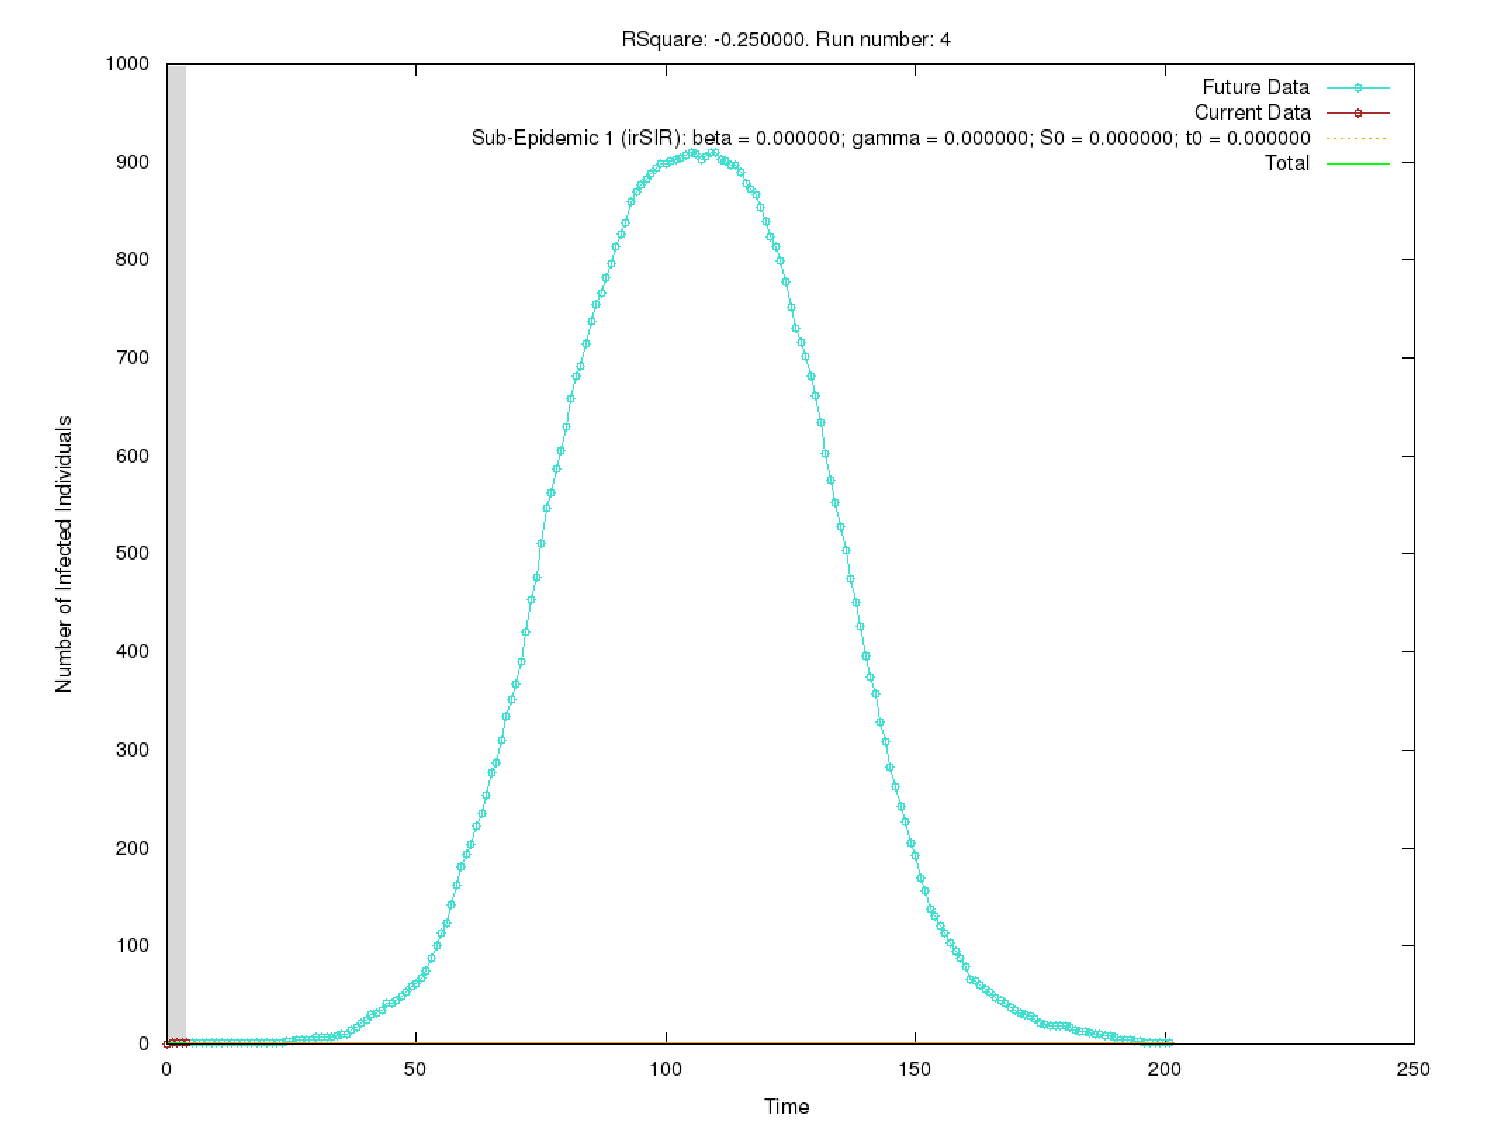
\includegraphics[width=8cm]{images/single/irsir1.png}
  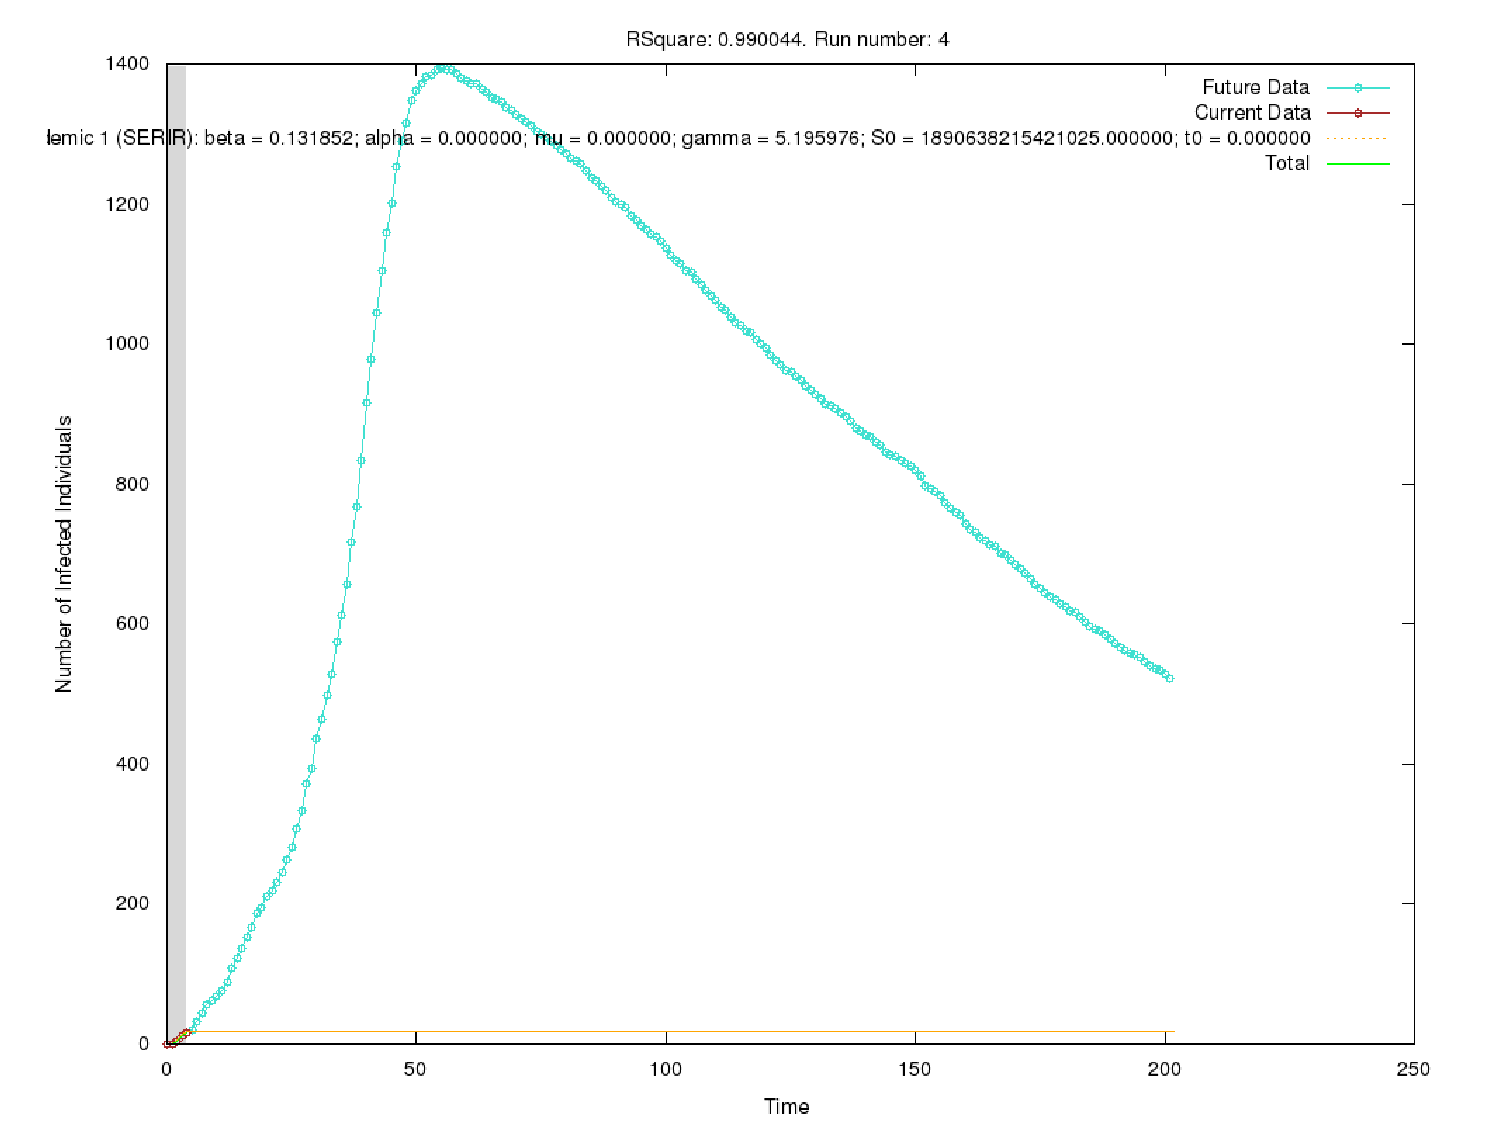
\includegraphics[width=8cm]{images/single/serir1.png}
\caption{Samples graphs of various candidate model fits (true
  parameter values in brackets): 1) SIR
  (0.0015,0.05,1000); 2) EXP (0.15,800); 3) SEIR (0.02,0.02,0.05,800);
  4) irSIR (0.0003,0.0001,2000); 5) SErIR (0.005,0.002,0.002,0.01,1500)}
\label{fig:single1}
  \end{figure}
\end{centering}


\begin{centering}
\begin{figure}[h!]
  \includegraphics[width=8cm]{images/single/ex1.png}
  \includegraphics[width=8cm]{images/single/ex2.png}
  \includegraphics[width=8cm]{images/single/ex3.png}
  \includegraphics[width=8cm]{images/single/ex4.png}
  \caption{Model fitting over time on an irSIR model with parameters of
    beta = 0.0001, gamma = 0.0005, and S0 = 2000}
\label{fig:single2}
  \end{figure}
\end{centering}

One important observation that was made when testing the single
epidemic fitting framework was that the optimisation procedure
occasionally settles on values widely outside of a realistic range
that still provide a good model fit. This was particularly prevalent
at earlier data points for the more complex models, possibly due to
the much larger parameter search space. Figure~\ref{fig:single3} shows
some examples of this problem. In the case of the first \emph{SErIR}
graph, the S0 value is found to be almost 17000000000, which greatly
differs from the true value of 1500. The algorithm is able to still
provide a decent fit by using very high recovery values (mu and
gamma). A solution to this problem that is explored in the next
chapter when fitting multiple epidemics is to bound the possible
parameter search space to a pre defined realistic range.

\begin{centering}
\begin{figure}[h!]
  \includegraphics[width=8cm]{images/single/bad1.png}
  \includegraphics[width=8cm]{images/single/bad2.png}
  \caption{Model fits of an SErIR and SEIR model where unrealistic
    values provide a decent model fit}
\label{fig:single3}
  \end{figure}
\end{centering}


\subsection{Unknown Model Types}
The next step in testing the model fitting framework is to assess how
well it is able to choose the correct model type for a given data set
when the model type is entirely unknown. At the start of the fitting
procedure, the best of twenty optimised fits are found for each
candidate model, and the model which produces the lowest \emph{AICc}
value is chosen as the correct model. To prevent the framework from
becoming stuck with the wrong model type early on in the fitting
process, we reconsider each candidate model every ten data points.

The model fitting framework still manages to produce a good model fit
for each of the tested synthetic data sets. In the case of the synthetic
\emph{SIR} data, the fitting framework is able to correctly select the
\emph{SIR} model. This is depicted in figure~\ref{fig:unknown1}, where
despite choosing to use an \emph{SErIR} model at one point during the
fitting procedure, the framework is able to correctly return to using
an \emph{SIR} model. It should be noted that the best fitting model
type might vary over the course of the run due to variation in the
data itself.

\begin{centering}
\begin{figure}[h!]
  \includegraphics[width=8cm]{images/single/unknown.png}
  \includegraphics[width=8cm]{images/single/unknown1.png}
  \includegraphics[width=8cm]{images/single/unknown2.png}
  \includegraphics[width=8cm]{images/single/unknown3.png}
  \caption{Fitting procedure on an SIR model where the model type is
    assumed to be unknown}
\label{fig:unknown1}
  \end{figure}
\end{centering}

Despite penalising more complex models using the \emph{AICc} criteria, the
fitting framework often selects an \emph{SIR} model in place of an
\emph{EXP} model. This is unsurprising, as the \emph{EXP} model is
simply a special case of the \emph{SIR} model when beta is very high
(and susceptible individuals therefore move into the infected
compartment almost instantly). Furthermore, we see in
figure~\ref{fig:unknown2} that the framework
often chooses between the \emph{SErIR} and \emph{SEIR} interchangeably. Again,
the two models are closely related. As mu tends to 0, the \emph{SErIR}
model tends to the equivalent \emph{SEIR} model. 


\begin{centering}
\begin{figure}[h!]
  \includegraphics[width=8cm]{images/single/unknownwrong1.png}
  \includegraphics[width=8cm]{images/single/unknownwrong2.png}
  \caption{Interchangeable selection of the similar SErIR and SEIR
    model types}
\label{fig:unknown2}
  \end{figure}
\end{centering}


Although all of the models can produce similar shapes due to their high level of
similarity, we would still expect the \emph{AICc} criteria to penalise
any model that is unecessarily complex such that the simplest model is
chosen. This case is only satisfied in the situation that a maximally
optimised fit is produced for each candidate model. However, by
choosing random parameters to start each optimisation, the
optimisation might return slightly sub optimal parameters some of the
time. For example, the best run from random parameters for an
\emph{SIR} model might produce an R Square of 0.97, whereas the run
using an \emph{SErIR} model might produce a fit of 0.99 simply as a
result of being seeded with better initial parameters. 

The problem of incorrect model selection might be countered
by using a greater number of random runs and by decreasing the error
tolerance of the Nelder-Mead algorithm to ensure that all model fits
find the global minimum rather than a similar local
minimum. Similarly, we might also increase the max number of
iterations allowed in the Nelder-Mead algorithm, but this limit is
not currently reached. However, these adjustments will drastically increase the amount of time taken for a full optimisation
run. This therefore represents an important trade off to be considered when deploying
the fitting framework. Another potential solution would be to use
alternative means of model selection. The \emph{AICc} score may not
sufficiently penalise more complex models when the difference in
number of parameters is minimal and the number of data points is
high. An alternative might be to simply select the model with the
fewest parameter that satisfies some desired fit value.


\subsection{CDC Influenza Data}
To put the model fitting framework to the test, we attempt to
characterise the CDC infected data for the H1N1 virus during 2013 to
2014. The fitting framework is able to choose and fit a model to the
data with very high accuracy, selecting the \emph{SIR} model for the
duration of the fitting procedure, and generating an R Square value of
over 0.99 consistently once the peak is reached. The predicted
trajectory of the epidemic matches the future data well.

\begin{centering}
\begin{figure}[h!]
  \includegraphics[width=8cm]{images/single/h1n1.png}
  \includegraphics[width=8cm]{images/single/h1n1b.png}
  \includegraphics[width=8cm]{images/single/h1n1c.png}
  \includegraphics[width=8cm]{images/single/h1n1d.png}
  \caption{Fitting procedure on the 2013-14 H1N1 CDC flu data}
\label{fig:unknown2}
  \end{figure}
\end{centering}

We go on to test the fitting framework on the AH3 virus during 2010 to
2011, but this time include the initial number of infected
individuals, I0, as an additional unknown parameter. Again, the
framework is able to characterise the data with a high R Square value
throughout. In this case, the type of model chosen changes during the
fitting, but settles on a high fitting \emph{SIR} model by the end.

\begin{centering}
\begin{figure}[h!]
  \includegraphics[width=8cm]{images/single/ah3.png}
  \includegraphics[width=8cm]{images/single/ah3b.png}
  \includegraphics[width=8cm]{images/single/ah3c.png}
  \includegraphics[width=8cm]{images/single/ah3d.png}
  \caption{Fitting procedure on the 2010-11 AH3 CDC flu data, with I0
    considered unknown}
\label{fig:unknown3}
  \end{figure}
\end{centering}


\subsection{Internet Epidemic Data}
In addition to conventional infectious disease epidemic data, we wish
to test how well the model fitting framework can characterise epidemic
phenomena on the internet. Figure~\ref{fig:fox1} shows the application
of the fitting framework to the number of daily \emph{BitTorrent}
downloads of the viral song ``\emph{The Fox (What does the Fox say?}''
between September 2013 and August 2014. The large peak corresponds to
the single release in Norway on October 11th 2013. The framework
detects and characterises the initial small peak accurately, and
adapts to characterise the overall peak as the fitting procedure
continues. By the end of the fitting, the framework has characterised
the data with an \emph{SErIR} model with an R Square value of 0.909.


\begin{centering}
\begin{figure}[h!]
  \includegraphics[width=8cm]{images/single/fox1.png}
  \includegraphics[width=8cm]{images/single/fox2.png}
  \includegraphics[width=8cm]{images/single/fox3.png}
  \includegraphics[width=8cm]{images/single/fox4.png}
  \caption{Fitting procedure on the 2013 viral hit, ``The Fox (What
    does the Fox say?)''}
\label{fig:fox1}
  \end{figure}
\end{centering}


\section{Chapter Summary}
In this section we have discussed the implementation and trial of an R
and C++ model fitting framework. The C++ framework is implemented from
scratch, using the Runge-Kutta method for solving ODEs, and the Nelder
Mead algorithm for optimisation. We assume that the transition
parameters and initial number of susceptibles, S0, are entirely
unknown, and also consider the case where I0 is known. We include five types of candidate
model and attempt to select the best fitting model using the
\emph{AICc} score, and show reasonable success. The framework is
tested using synthetic data, real influenza data, and
\emph{BitTorrent} download data. In all cases we are able to provide a
model with a high R Square fit.
